\section{The Unilateral Multi-Downgrade Attack} \label{sec:umd-attack}

Beyond rediscovering known attacks, the compound-key decomposition enabled by our three-tier oracle uncovers a novel attack on Bluetooth Classic that we call the Unilateral Multi-Downgrade~(UMD) attack.
In this attack, an adversary repeatedly downgrades the key length on \emph{one} side of a BC session and recombines the recovered key fragments to reconstruct the full session key.

\subsection{Attack Cost}

The attacker chooses a downgrade factor $n$ (the number of downgrade steps).
At each step, the attacker forces the peripheral to use a session key of $128/n$ bits and brute-forces that fragment.
The total cost is:
\begin{equation} \label{eq:umd-cost}
    C(n) = n \cdot 2^{128/n}
\end{equation}

\begin{table}[t]
    \centering
    \caption{UMD attack cost $C(n)$ for selected downgrade factors}
    \label{tab:umd-cost}
    \begin{tabular}{rrl}
        \toprule
        $n$ & $C(n)$ & Comment \\
        \midrule
        1 & $2^{128}$ & No downgrade (infeasible) \\
        2 & $2^{65}$ & Two half-key fragments \\
        4 & $2^{34}$ & Four quarter-key fragments \\
        8 & $2^{19}$ & Eight 2-byte fragments \\
        16 & $2^{12}$ & Sixteen 1-byte fragments (optimal) \\
        \bottomrule
    \end{tabular}
\end{table}

\autoref{tab:umd-cost} lists $C(n)$ for selected values.
At $n=16$, the attacker recovers a 128-bit session key with cost $2^{12}$---a factor of $2^{116}$ reduction compared to direct brute-force.

\subsection{Attack Trace}

We illustrate the attack with $n=4$ (\autoref{fig:bc-umd}).
Consider a central device that only accepts 16-byte keys and a peripheral device that supports 1--16~byte keys.
Under normal conditions, they negotiate a 16-byte session key, making brute-force infeasible.

\begin{figure}[t]
    \centering
    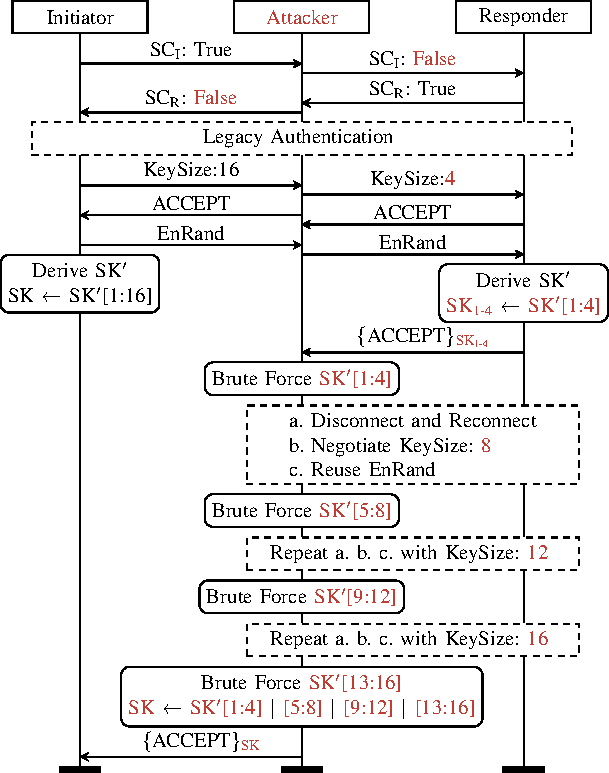
\includegraphics[width=0.945285\columnwidth]{img/umd-attack}
    \caption{Attack flow of UMD attack on BC session establishment}
    \label{fig:bc-umd}
\end{figure}

The attacker proceeds as follows:
\begin{enumerate}[leftmargin=*]
    \item \textbf{Downgrade to Legacy.} The attacker forces both devices into a Legacy session by manipulating feature exchange messages.
    \item \textbf{First fragment.} The attacker induces the peripheral to use a 4-byte session key and brute-forces the first 4~bytes of the session key ($2^{32}$ operations).
    \item \textbf{Subsequent fragments.} The attacker repeats the session establishment three more times, each time recovering an additional 4-byte fragment.
    \item \textbf{Reconstruction.} The attacker combines the four fragments to recover the complete 16-byte session key.
\end{enumerate}

The key insight is that the session key $SK'$ is derived from the link key $LK$ and the $ACO$ value, both of which persist across sessions.
Each truncated session key $SK = \text{resize}(SK', N_i)$ exposes a different prefix of $SK'$, and the attacker accumulates these prefixes across sessions.

\subsection{Discovery via MDerive}

The UMD attack is not an artifact of manual analysis; it is a direct product of the recursive decomposition enabled by \TFact{MDerive}.
In a standard \Tamarin{} model, the full-length session key $SK'$ is an atomic 128-bit term that the Dolev-Yao attacker cannot decompose---the perfect encryption assumption treats $SK'$ as opaque.
EntropyVerif changes this in three steps:

\begin{enumerate}[leftmargin=*]
    \item \textbf{Derivation fact generation.}
    When the \Tterm{ResizeSK} rule truncates $SK'$ to a negotiated length (e.g., $N_1$), EntropyVerif emits $\text{\TFact{MDerive}}(l(l(SK')), \text{resize}(SK', N_1))$ and marks $l(l(SK'))$ as low-entropy via \TFact{EntropyLow}.
    \item \textbf{Cross-session chaining.}
    The \emph{message-derivation} oracle chains derivation facts across sessions: the first session exposes $\text{\TFact{MDerive}}(l(l(SK')), SK_1)$; the second session, with a different truncation level, exposes $\text{\TFact{MDerive}}(r(l(SK')), SK_2)$.
    Both facts are linked to the same underlying $SK'$.
    \item \textbf{Fragment recovery.}
    The \emph{relationship-breaking} oracle strips known fragments from compound derivations, and the \emph{value-breaking} oracle recovers each 1-byte fragment individually.
    \Tamarin{}'s backward search composes these steps and outputs the complete attack trace automatically.
\end{enumerate}

\noindent
This trace could not have been found without the recursive composition of all three oracle tiers: value-breaking alone cannot handle compound keys; relationship-breaking alone cannot chain across sessions; message-derivation alone cannot recover individual fragments.
The UMD attack thus serves as a concrete proof-of-concept for the necessity of the three-tier design.

\subsection{Impact Analysis}

The UMD attack differs from the KNOB attack in three respects that make it more concerning in practice:
\begin{enumerate}[leftmargin=*]
    \item \textbf{Asymmetric prerequisite.}
    KNOB requires \emph{both} central and peripheral to accept short keys.
    UMD only requires the \emph{peripheral} to accept short keys; the central device may enforce maximum-length keys throughout.

    \item \textbf{Asymmetric remediation cost.}
    Central devices (smartphones, laptops) receive regular OTA updates.
    Peripheral devices (IoT sensors, audio accessories, automotive modules) often lack firmware upgrade paths, making it infeasible to patch the installed base.

    \item \textbf{Residual risk after specification updates.}
    Even if the Bluetooth specification raises the minimum key length to 7~bytes, the UMD attack remains viable: with $n=8$ downgrade steps (each yielding a 2-byte fragment from a 16-byte key), the cost is $C(8) = 8 \cdot 2^{16} = 2^{19}$, still a factor of $2^{109}$ below direct brute-force of $2^{128}$.
\end{enumerate}

\subsection{Responsible Disclosure}

We reported this vulnerability to the Bluetooth Special Interest Group~(SIG) security team on July~15, 2024.
In their February~7, 2025 response, the SIG stated that ``the scenario posited for identifying the session key used during BR/EDR encryption establishment appears much more practical'' than previously known attacks.
The SIG is conducting a detailed analysis and will provide further feedback.

